This chapter will go over the results of the manufacturing of the DAQ system as well as its performance and reliability during SDM-23's track days.

\section{System Manufacturing}
Although the DAQ system was designed with a Rear I/O box in mind, this box was never designed nor manufactured due to time constraints, which severely affected our ability to collect data at the rear of the car.
The design deadline set by the team was also not respected.
\subsection{Wiring Manufacturing}
The original design for the DAQ system utilised Binder 719 connectors, which were selected because they came in panel-mount versions and because they are prevalent in AiM systems.
These were assembled by soldering wires to the solder cups on the connectors.
Although they were small and lightweight, they were very difficult and time-consuming to solder and assemble, and were prone to creating shorts in the wires due to soldering errors.
\vspace{1em}

As such, the decision was made partway through the manufacturing phase to switch over to DTM connectors for all connections, which required crimping terminals onto wires instead of soldering them.
Although DTM connectors are much larger (a size comparison with a DT connector is shown in Figure \ref{fig:binderbad}), their crimp termination meant that assembling these connectors are much easier and less prone to human error.
It should be noted that although this delayed the completion of the DAQ system as the PCB enclosures needed to be redesigned for the larger connectors and for the DTM connectors to arrive, this greatly increased the reliability of the DAQ system and made it faster and easier to manufacture the rest of the system.
\begin{figure}[H]
    \centering
    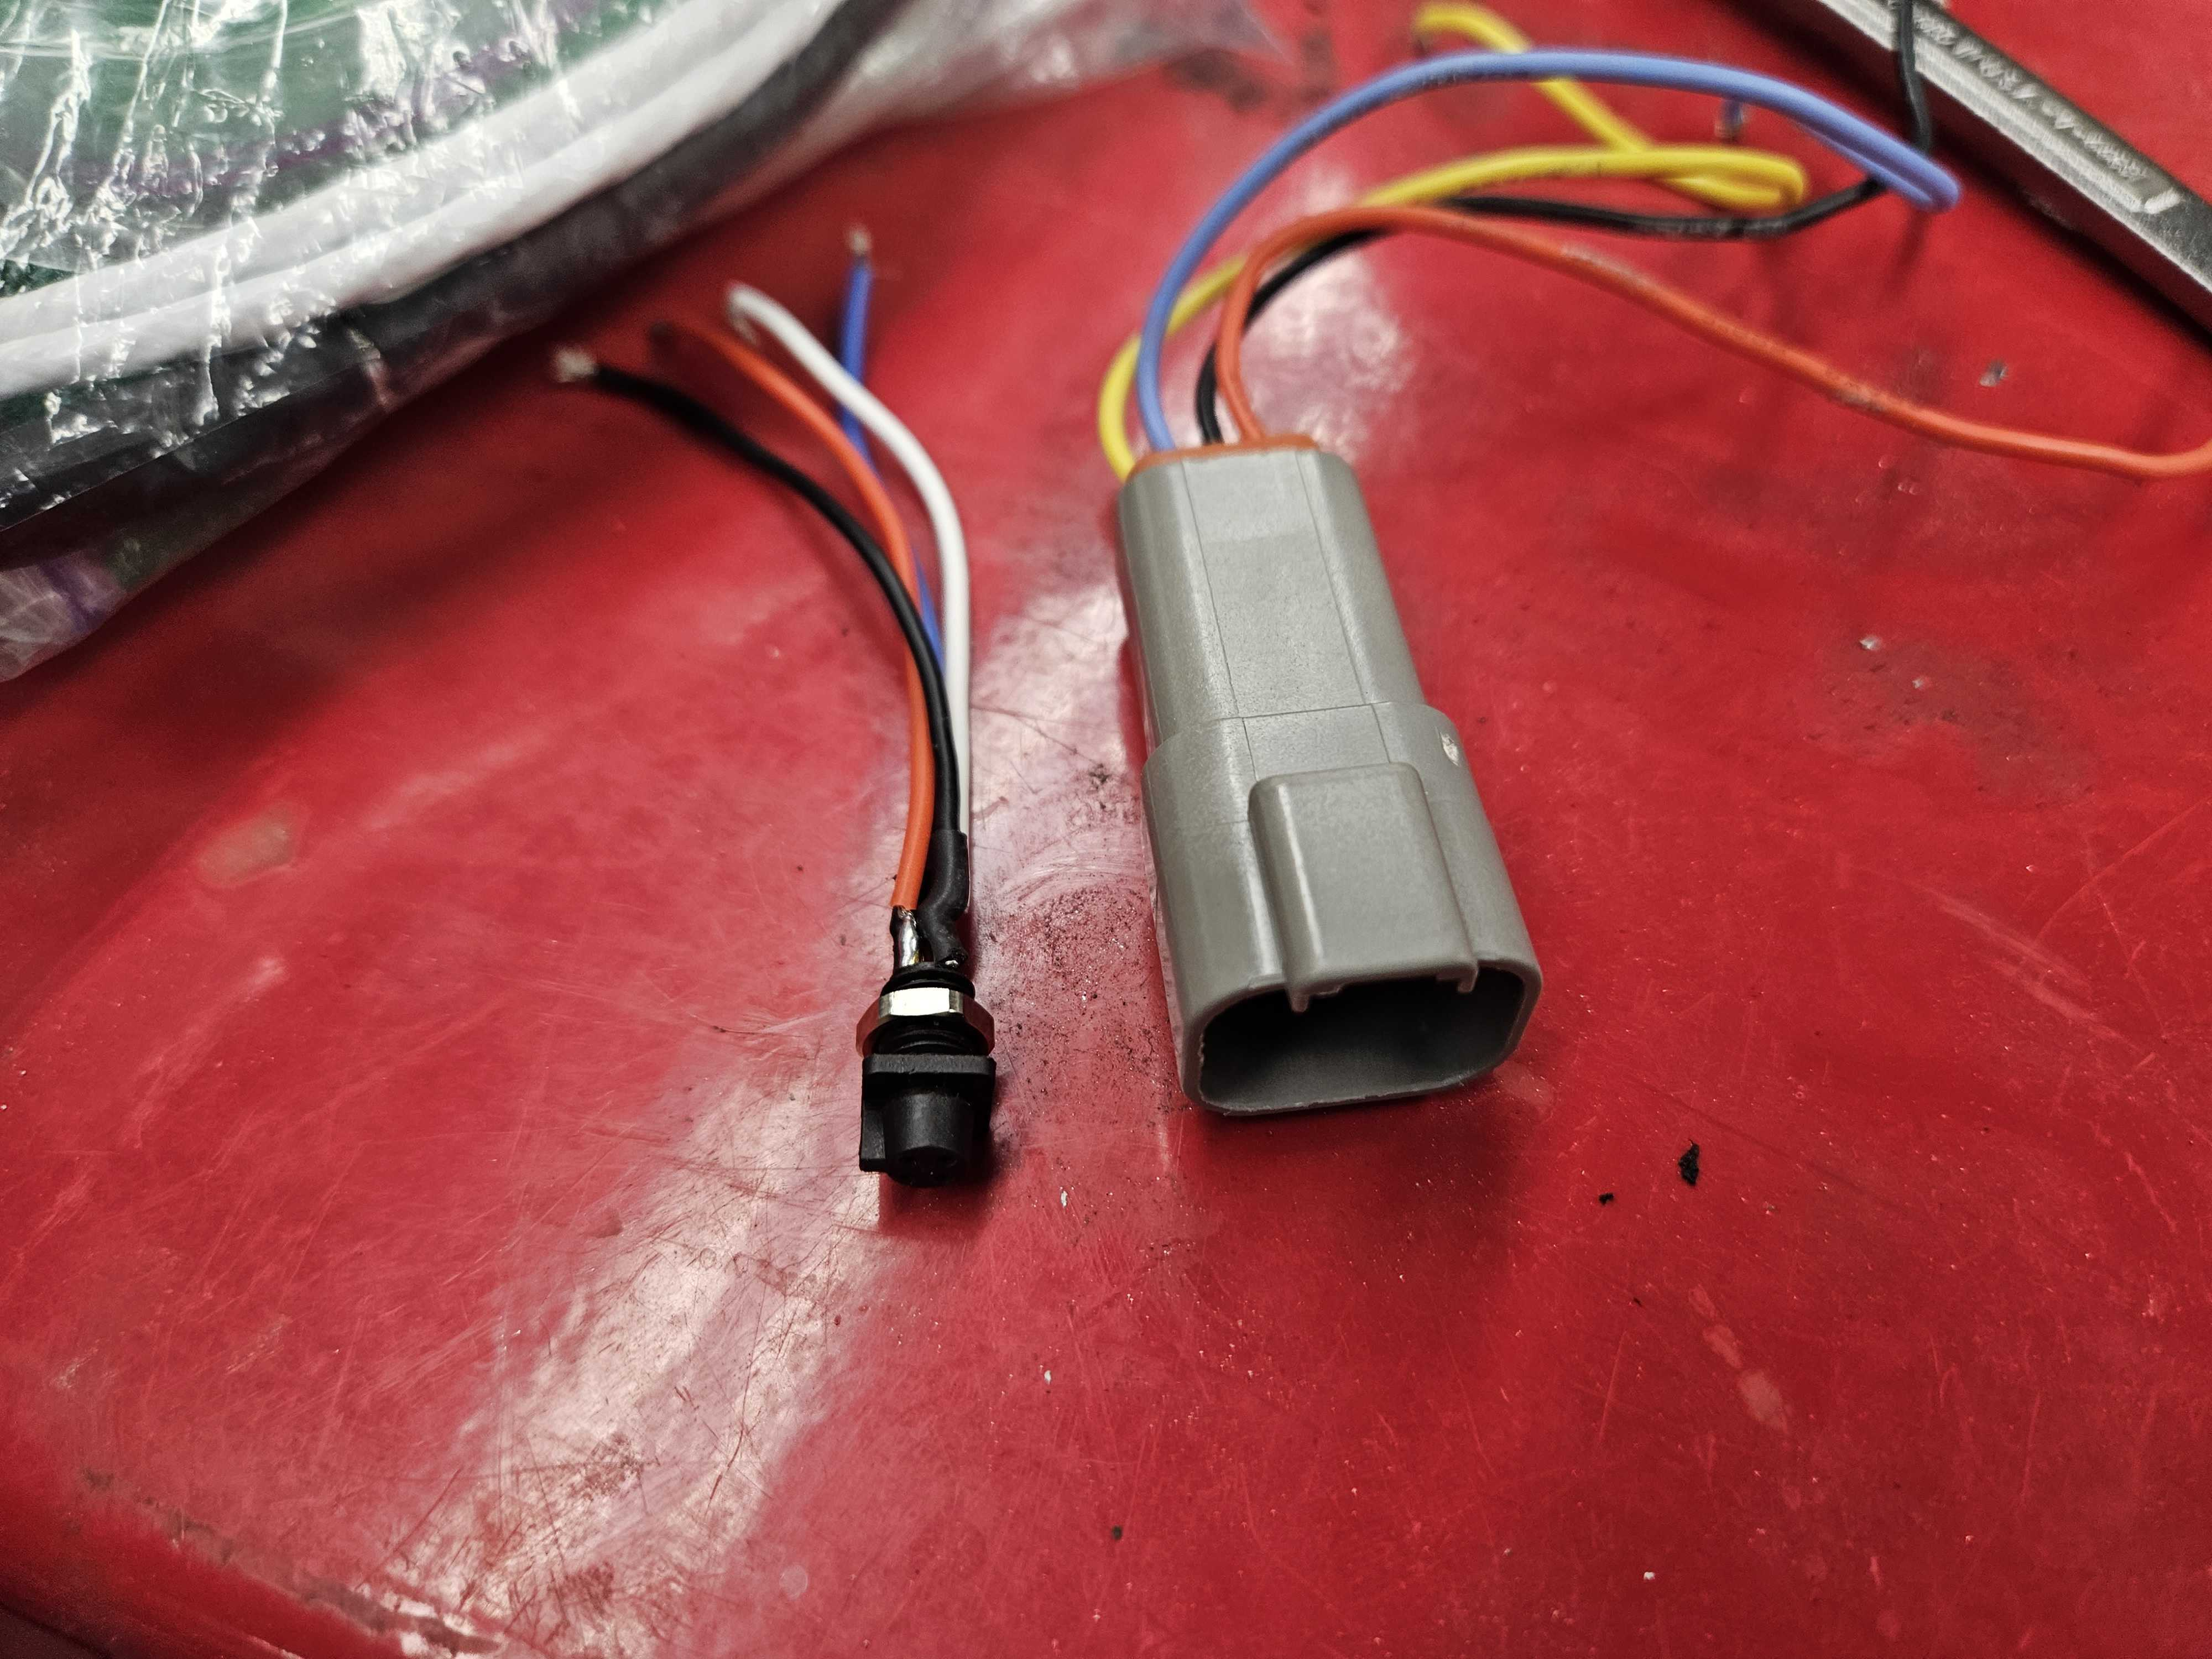
\includegraphics[width=4in]{images/binder.jpg}
    \caption{Size comparison between a Binder 719 and a DT connector}
    \label{fig:binderbad}
\end{figure}

\subsection{Sensor Calibration}
\subsubsection{Brake Pressure Sensor}
The transfer function for the brake pressure sensor has been given by Honeywell in the product datasheet.
However since a voltage divider was used to step down the output from the brake pressure sensor into a suitable range for the Teensy, this must be accounted for before using the provided transfer function.
First, the raw ADC value is converted to volts:
\begin{gather}
    V_{3.3}(a) = a\cdot \frac{3.3}{1023}
\end{gather}
This is converted into a 5V range by using the inverse of the voltage divider (Using 6.8k$\Omega$ for $R_1$ and 10k$\Omega$ for $R_2$):
\begin{gather}
    V_5(v) = 1.68\cdot v
\end{gather}
Once a voltage value in the range $[0,5]$ has been obtained we can then use the transfer function in Equation \ref{eq:bps} to get a brake pressure value.

\subsubsection{Brake Rotor Temperature Sensor}
Initially, the setup code for the MLX90614 would set the emissivity value of the sensor on every startup.
However, this would cause the sensor to sometimes read negative values during the duration of a run, which is obviously not correct, an example seen in Figure \ref{fig:hehehehehe}.
\begin{figure}[H]
    \centering
    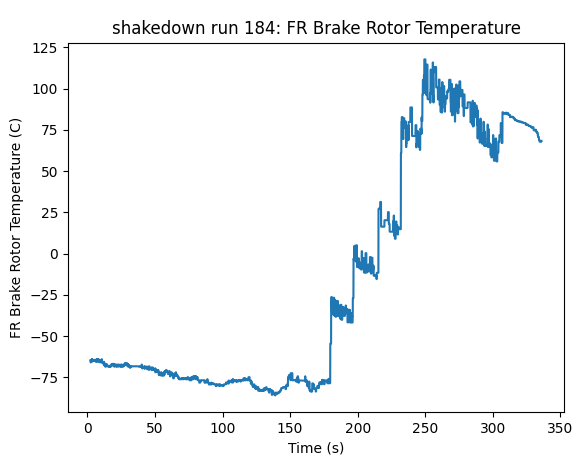
\includegraphics[width=3.5in]{images/negativetemp.png}
    \caption{MLX90614 reading negative temperatures}
    \label{fig:hehehehehe}
\end{figure}
Upon further investigation, an issue on the MLX90614 library's GitHub page found that power cycling the sensor after changing the emissivity would solve the issue.
It was also determined that the emissivity value used by the sensor is saved internally in the sensor, so there is no need to set the emissivity every time the DAQ system turned on.
\vspace{1em}

After removing the emissivity line, the MLX90614 no longer read negative values, with the only issue remaining is that the sensor's object temperature reading would spike to a five figure number.
As of the time of writing, this has not been solved yet.
A quick fix that can be applied during data processing is to throw out the spike.
\begin{figure}[H]
    \centering
    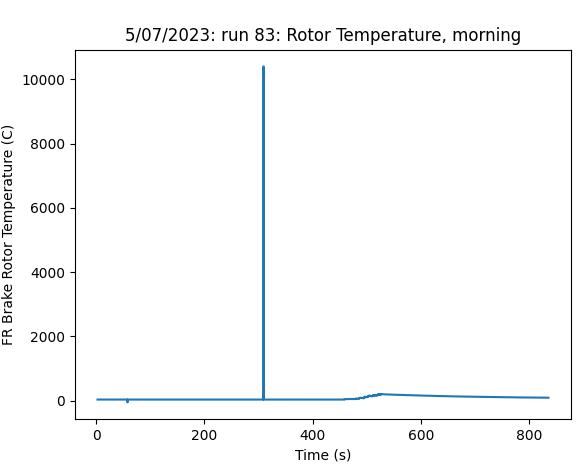
\includegraphics[width=3.5in]{images/hot.png}
    \caption{Temperature spike in the MLX90614 output}
    \label{fig:hot}
\end{figure}
\subsubsection{Damper Potentiometer}
Since the same potentiometer model was used from SDM-22, the transfer function created for that year was carried over, with the only addition being that the units changed from inches to millimeters.
\begin{gather}\label{eq:dptf}
    P(a) =  0.053440584\times a
\end{gather}
Equation \ref{eq:dptf} shows the transfer function $P(a)$ that outputs the potentiometer's current position in millimeters given the 10-bit ADC value $a$.
During the data processing stage, damper displacement and velocity would be calculated using this value.
\subsubsection{Gyroscope}
At the time of writing, the gyroscope settings have not been sufficiently tuned to produce consistent angular position data due to lack of time.
The gyroscope debugger requires more work in order to be useful, as there was a significant delay in moving the IMU unit and the data showing up on the debugger.
\vspace{1em}

Another consideration that should be made is how the IMU is mounted in the car, as the IMU had a lot of rotational slack.
\subsubsection{Steering Angle Sensor}
From testing the rotary potentiometer, we found that it had a linear slope and did not have a hard stop.
Once it was installed onto the steering rack, we found the following values for the steering wheel's center, right, and left positions:
\begin{table}[H]
    \centering
    \begin{tabular}{|c|c|}
        \hline
         Steering Wheel Angle & ADC output of potentiometer \\
        \hline
         center & 102 \\
         90 degrees right & 337 \\
         90 degrees left & 902 \\
        \hline
    \end{tabular}
    \caption{Calibration values for the Steering Angle Sensor}
    \label{tab:sas}
\end{table}
As seen in Table \ref{tab:sas}, the potentiometer ``overflows'' when turning the wheel left.
As such the transfer function for the steering angle sensor would need to be piecewise:
\begin{gather}
    A(a) = \begin{cases} 
      0.392\cdot a - 42.176 & a \leq 500 \\
      0.392\cdot (a - 1024) - 42.176 & a > 500 \\
   \end{cases}
\end{gather}
$A(a)$ returns a value in degrees where $a$ is the ADC value of the rotary potentiometer.
A positive value would indicate turning right, while a negative value would indicate turning left.
Zero indicates the steering wheel is centered.

\subsubsection{Strain Gauges}
At the time of writing, the strain gauge output have not been used or validated.
There were also issues with the strain gauges, likely stemming from manufacturing errors in either the bonding process or the strain gauge amplifier assembly.
The output from the front left strain gauge on the push rod was wildly inconsistent.
In other instances, the strain gauge output would stick at $50\%V_{in}$. 

\section{System Performance}
\subsection{Electrical Performance}
Throughout SDM-23 testing, electrical reliability was the DAQ system's greatest weakness.
Poor and/or inconsistent solder joints in the PCBs would result in either loss of power in some boxes or loss of data transmission, both cases severely affecting data collection during track days.
Loss of power and/or data transmission was detected by inspection of the summary files, finding plateaus in the data (Figure \ref{fig:los} demonstrates this), or by visual inspection of the box (if a Teensy LED for a box was not lit, this would usually indicate power loss).
\begin{figure}[H]
    \centering
    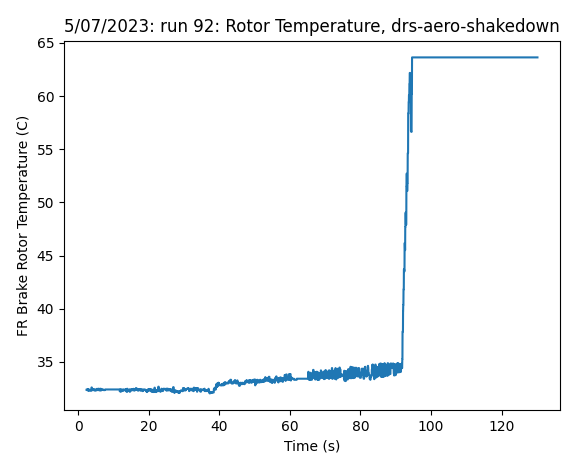
\includegraphics[width=4.5in]{images/data-loss.png}
    \caption{Instance of loss of power/data transmission by the Front IO box}
    \label{fig:los}
\end{figure}
In general, these were able to be diagnosed via continuity and voltage checks with a multimeter.
\vspace{1em}

Early on in SDM-23 testing, CAN data would occasionally drop from the driver dashboard.
This was easily fixed by removing the terminating resistor on the ECU CAN transceiver in the Main box.

\subsection{Mechanical Performance}
The mechanical aspect of the DAQ system worked as intended, as all the sensor mounts were able to hold up during track days.
One area for improvement would be to design more robust PCB enclosures, as it was difficult to plug or unplug connectors because if too much force was used the enclosure could shatter, so to avoid that occurring the receptacle would be held while plugging/unplugging the connector.

\subsection{Software Performance}
In most cases, the DAQ system's software worked as intended.
However, there were instances where the software failed due to relatively simple errors.
\vspace{1em}

One software fault was selecting the wrong Serial port to use for communication with the GPS module, which caused us to not collect any GPS data during one of the track days.
Another software fault was not logging steering angle data to the SD card.
Both of these faults could've been easily caught in a software review.
\vspace{1em}

A third software fault was not logging GPS position data and timestamps to a sufficient enough precision.
In the first case, this caused the GPS position data to be inaccurate and effectively useless.
The second case would cause issues when doing any calculations with a difference between consecutive timestamps, as there would be occasional duplicate timestamps.
Both cases were solved by logging these channels with additional precision: GPS position data would be logged to four decimal places while timestamps would be logged to three decimal places.
